\subsection{\Acl{MC}} 
\tododone[inline]{Proofreading of Benni \& JC}
The \acf{MC} method \cite{Marching2006} takes as an input a set of scalar function values on a Cartesian mesh and extracts an approximate isosurface in the form of a mesh of triangles. The method starts by dividing the space into cubes with the set of function values as cube vertices. These values are determined to be above or below the desired isovalue. According to which corners are set to be above or below, the corner configuration is then mapped to a polygon inside the cube, with vertices on the cube's edges. On an edge between a vertex above and a vertex below the desired isovalue, the exact location of the surface is determined via linear interpolation. Then this location is set as the polygon's vertex on that edge. A result of the \ac{MC} algorithm is shown in \autoref{fig:bunny}.

\begin{figure}
\centering
   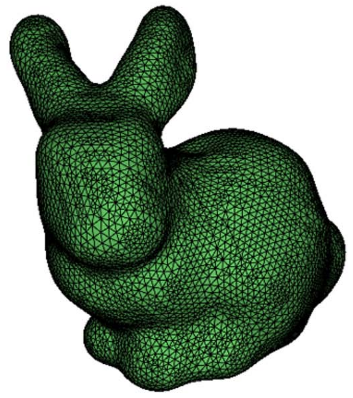
\includegraphics[width=.25\textwidth]{Pictures/SurfaceReconstruction/Bunny}
   \caption{The famous Stanford Bunny, a popular computer graphics test object, here after application of \ac{MC}. Figure from \cite{}. }
   \label{fig:bunny}
\end{figure}
\todourgent[inline,author=Benni]{Reference to \cite{Hermite2002} in \autoref{fig:bunny} was wrong! Fix this -> JC}

\subsubsection{The \acl{MC} cases}
Since there are 8 vertices on each cube, either above or below the isovalue (with equality falling to one of these categories), $2^8=256$ possible polygon configurations exist. However, many of these can be constructed by rotating or reflecting other polygons. Therefore 15 base cases which represent all the surface polygons of the \acl{MC} are sufficient to take into consideration. \autoref{fig:MC_basecase} shows how these base cases look like, we can notice that they are composed of triangles. 

\begin{figure}
\centering
   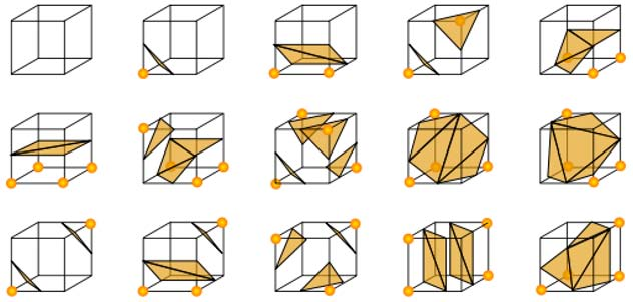
\includegraphics[width=.5\textwidth]{Pictures/cubes.pdf}
   \caption{The base cases of \ac{MC}. These are drawn with each polygon vertex intercepting its edge in the middle between the cube's corners, as in the case when the isovalue is exactly halfway between the function values at the vertices. Figure from \cite{Marching2006}.}
   \label{fig:MC_basecase}
\end{figure}

\subsubsection{Cracks and ambiguities}
The original algorithm presents two main problems. Firstly, it guarantees neither correctness nor topological consistency, which means that holes may appear on the surface due to inaccurate base case selection. The second problem is ambiguity, which appears when two base cases are possible and the algorithm chooses the incorrect one, or cannot decide on one. There are many extended \ac{MC} algorithms that tackle the problems of the original one, getting rid of the ambiguities and providing correctness (see for example \cite{ExtendedMC}).
